\subsection{Discover the Fun Uses of a Smith Chart!}

\begin{tcolorbox}[colback=gray!10, colframe=black, title=E9G05]

Which of the following is a common use for a Smith chart? 
\begin{enumerate}
    \item \textbf{A} Determine the length and position of an impedance matching stub
    \item B Determine the impedance of a transmission line, given the physical dimensions
    \item C Determine the gain of an antenna given the physical and electrical parameters
    \item D Determine the loss/100 feet of a transmission line, given the velocity factor and conductor materials
\end{enumerate} \end{tcolorbox}

\subsubsection{Explanation of Concepts}

The Smith chart is a graphical tool primarily used in radio frequency (RF) engineering for solving problems related to transmission lines and matching circuits. Its applications include impedance matching, analyzing complex impedances, and visualizing the relationships between voltage, current, and impedance.

1. \textbf{Impedance Matching:}: This is crucial in RF systems to ensure maximum power transfer from a source to a load. The Smith chart helps visualize how impedance changes with frequency and how various matching strategies—like stubs and transformers—can be employed.

2. \textbf{Transmission Lines:}: The chart helps in understanding how load impedance variations affect the reflection coefficient and voltage standing wave ratio (VSWR), which are fundamental to transmission line performance.

3. \textbf{Stub Matching:}: This method involves adding a reactive component (a stub) in parallel or series to achieve an optimal impedance at a specific frequency. The Smith chart allows one to plot the existing impedance and to quickly visualize the necessary adjustments.

4. \textbf{Calculations:}: To use a Smith chart for determining the length and position of an impedance matching stub:
   - First, plot the load impedance on the Smith chart.
   - Locate the point representing the normalized load impedance.
   - Move along the constant reactance circle (in the direction of increasing frequency) to find the point where the desired impedance is located.
   - The intersection gives the required length and position of the stub.

\subsubsection{Additional Notes}

The Smith chart simplifies the process of impedance matching significantly, and its versatility makes it a staple in RF design, particularly for antennas and transmission lines. Understanding how to read and utilize the chart can greatly enhance one’s capability in RF engineering.

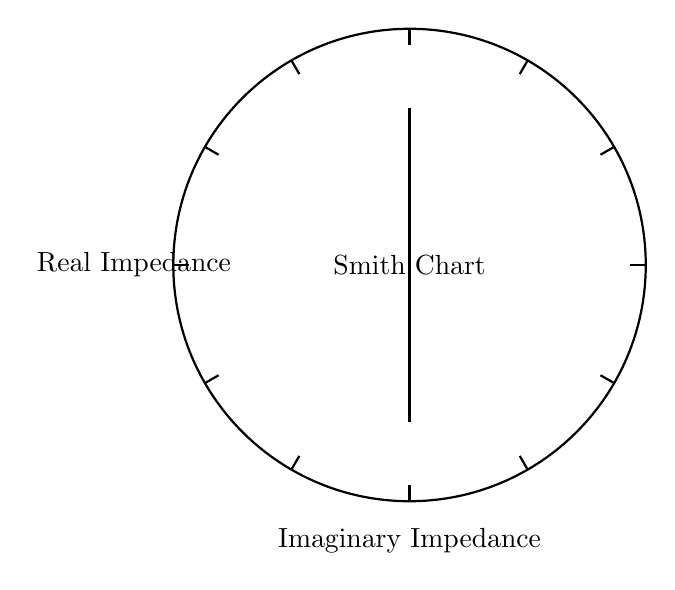
\begin{tikzpicture}
    \draw[thick] (0,0) circle(3);
    \foreach \i in {0,30,...,360} {
        \draw[thick] (\i:2.8) -- (\i:3);
    }
    \foreach \i in {0,1,2,3} {
        \draw[thick] (0,-2+\i) -- (0,-1+\i);
    }
    \node at (0,0) {Smith Chart};
    \node at (-3.5,0) {Real Impedance};
    \node at (0,-3.5) {Imaginary Impedance};
\end{tikzpicture}
